\documentclass[a4]{article}

\pagestyle{empty}
\usepackage[top=10mm,bottom=10mm,left=5mm,right=5mm]{geometry}
\usepackage{tikz}
\usetikzlibrary{
    decorations.markings,
    decorations.pathmorphing,
    decorations.text,
}
\usepackage{graphicx}
\usepackage{contour}
\contournumber{64}

% FONTS
\usepackage{addfont}
\addfont[1]{OT1}{hge}{\textgothic}
\usepackage{fontspec}
\newfontface\textblack{QTHelvet-Black}
\usepackage{cabin}

\begin{document}
\noindent\begin{tikzpicture}
    % BORDER
    \draw[dashed] (-100mm,-100mm) rectangle (100mm,100mm);
    \draw[dashed] (0,0) circle (100mm);
    \draw[dashed] (0,0) circle [radius=3mm];
    \draw[dashed] (0,0) circle [radius=18mm];
    
    % NUMBERS
    % Background
    \draw[fill=black,draw=white,line width=1.4mm]
        (180:72mm) -- (180:88mm) arc (180:360:88mm)
        (360:88mm) -- (360:72mm) arc (360:180:72mm);
    % Numerals
    \contourlength{0.1mm} % set to one 7th (scale) of the desired width
    \foreach \angle/\label/\xscale in {%
            270/0/1,255/1/1,240/2/1,225/3/1,210/4/1,195/5/1,%
            180/6/1,165/7/1,150/8/1,135/9/1,120/X/1,105/3/-1%
    } {
        \node[rotate=\angle-90,scale=7,inner sep=0pt,xscale=\xscale]
            at (\angle:80mm-.3mm) {\contour{white}{\label}};
        \node[rotate=\angle+90,scale=7,inner sep=0pt,xscale=\xscale]
            at (\angle-180:80mm-.3mm) {\contour{white}{\label}};
    }
    % Little Circles
    \foreach \angle in {-90,-75,...,255} { % 24ths
        \draw[fill,draw=white,line width=.6mm]
            (\angle+7.5:80mm) circle [radius=1.5mm];
    }
    % Borders
    \draw [line width=2mm] (0,0) circle [radius=90mm-1mm];
    \draw [line width=2mm] (0,0) circle [radius=70mm+1mm];

    % FACE
    \newcommand{\insR}{22mm}
    \newcommand{\midR}{32mm}
    \newcommand{\outR}{57mm}
    % Rim
    \draw[line width=0.3mm] (0,0) circle (\outR-2.3mm-1.3mm);
    \foreach \angle in {0,7.5,...,353.5} {
        \draw[line width=0.3mm]
            (\angle:\outR-1.3mm) -- (\angle:\outR-1.3mm-2.3mm)
            (\angle+3.75:\outR-1.3mm) -- (\angle+3.75:\outR-1.3mm-1.15mm);
    }
    % Sectors
    \foreach \lcolor/\lwidth in {black/2.6mm,white/2mm} {
    \begin{scope}[every path/.style={draw=\lcolor,line width=\lwidth}]
        \draw (180:\insR)   -- (180:\outR)   arc(180:150:\outR)     --
              (150:\outR)   -- (150:\midR)   arc(150:127.5:\midR)   --
              (127.5:\midR) -- (127.5:\outR) arc(127.5:90:\outR)    --
              (90:\outR)    -- (90:\midR)    arc(90:67.5:\midR)     --
              (67.5:\midR)  -- (67.5:\outR)  arc(67.5:0:\outR)      --
              (0:\outR)     -- (0:\insR)     arc(0:180:\insR)       ;
        \draw (0:\insR)     -- (0:\outR)     arc(0:-60:\outR)       --
              (-60:\outR)   -- (-60:\insR)   arc(-60:0:\insR)       ;
        \draw (300:\insR)   -- (300:\midR)   arc(300:240:\midR)     --
              (240:\midR)   -- (240:\outR)   arc(240:180:\outR)     --
              (180:\outR)   -- (180:\insR)   arc(180:300:\insR)     ;
        \draw (150:\midR)   -- (150:\outR)   arc(150:127.5:\outR)   --
              (127.5:\outR) -- (127.5:\midR) arc(127.5:150:\midR)   ;
        \draw (67.5:\midR)  -- (67.5:\outR)  arc(67.5:90:\outR)     --
              (90:\outR)    -- (90:\midR)    arc(90:67.5:\midR)     ;
    \end{scope}
    }
    % (Cover up external lines)
    \newcommand{\clearcol}{white}
    % \renewcommand{\clearcol}{green}
    \draw[line width=1mm,draw=\clearcol] (0,0) circle (\outR+1.15mm);
    \draw[line width=1mm,draw=\clearcol] (0,0) circle (\insR-1.15mm);
    \path[fill=\clearcol]
        (300:\midR) -- (300:\outR+1.3mm) arc(300:240:\outR+1.3mm) --
        (240:\outR+1.3mm) -- (240:\midR) arc(240:300:\midR);
    % Labels
    \foreach \phi/\label in {180/Write,153.75/Morn,123.75/Read,93.75/Noon,%
        48.75/Work,345/Eve,225/Sleep} {
        \path[postaction={decorate,decoration={text align={center},%
            raise={4mm},text along path,text={|\huge\textgothic|\label}}}]
            (\phi:\outR) arc (\phi:\phi-30:\outR);
    }

    % PANEL
    % signature
    \node at (270:39mm) {\includegraphics[width=30mm]{sign.png}};
    % title
    \path[postaction={decorate,decoration={text align={center},%
        text along path,text={|\Large\textblack|24 HOUR WORLD CLOCK}}}]
        (240:65mm) arc (240:300:65mm);
    % offset information and blank
    \path[postaction={decorate,decoration={text align={right},text along
        path,text={|\sffamily\small|RIM OFFSET}}}]
        (240:54mm) arc (240:260:54mm);
    \draw[dashed,line width=0.3mm]
        (262.5:58mm) -- (262.5:48mm) arc(262.5:277.5:48mm) --
        (277.5:48mm) -- (277.5:58mm) arc(277.5:262.5:58mm) ;
    \path[postaction={decorate,decoration={text align={left},text along
        path,text={|\sffamily\small|FROM LOCAL}}}]
        (280:54mm) arc (280:300:54mm);
    \fill (270:58mm) -- (271:60mm) -- (269:60mm);

    % THE EXAMPLE
    \path[postaction={decorate,decoration={text align={center},text along
        path,text={|\sffamily\small|+24/0/-24}}}]
        (262.5:54mm) arc (262.5:277.5:54mm);
    \fill (270:58mm) -- (271:56mm) -- (269:56mm);
\end{tikzpicture}

\noindent
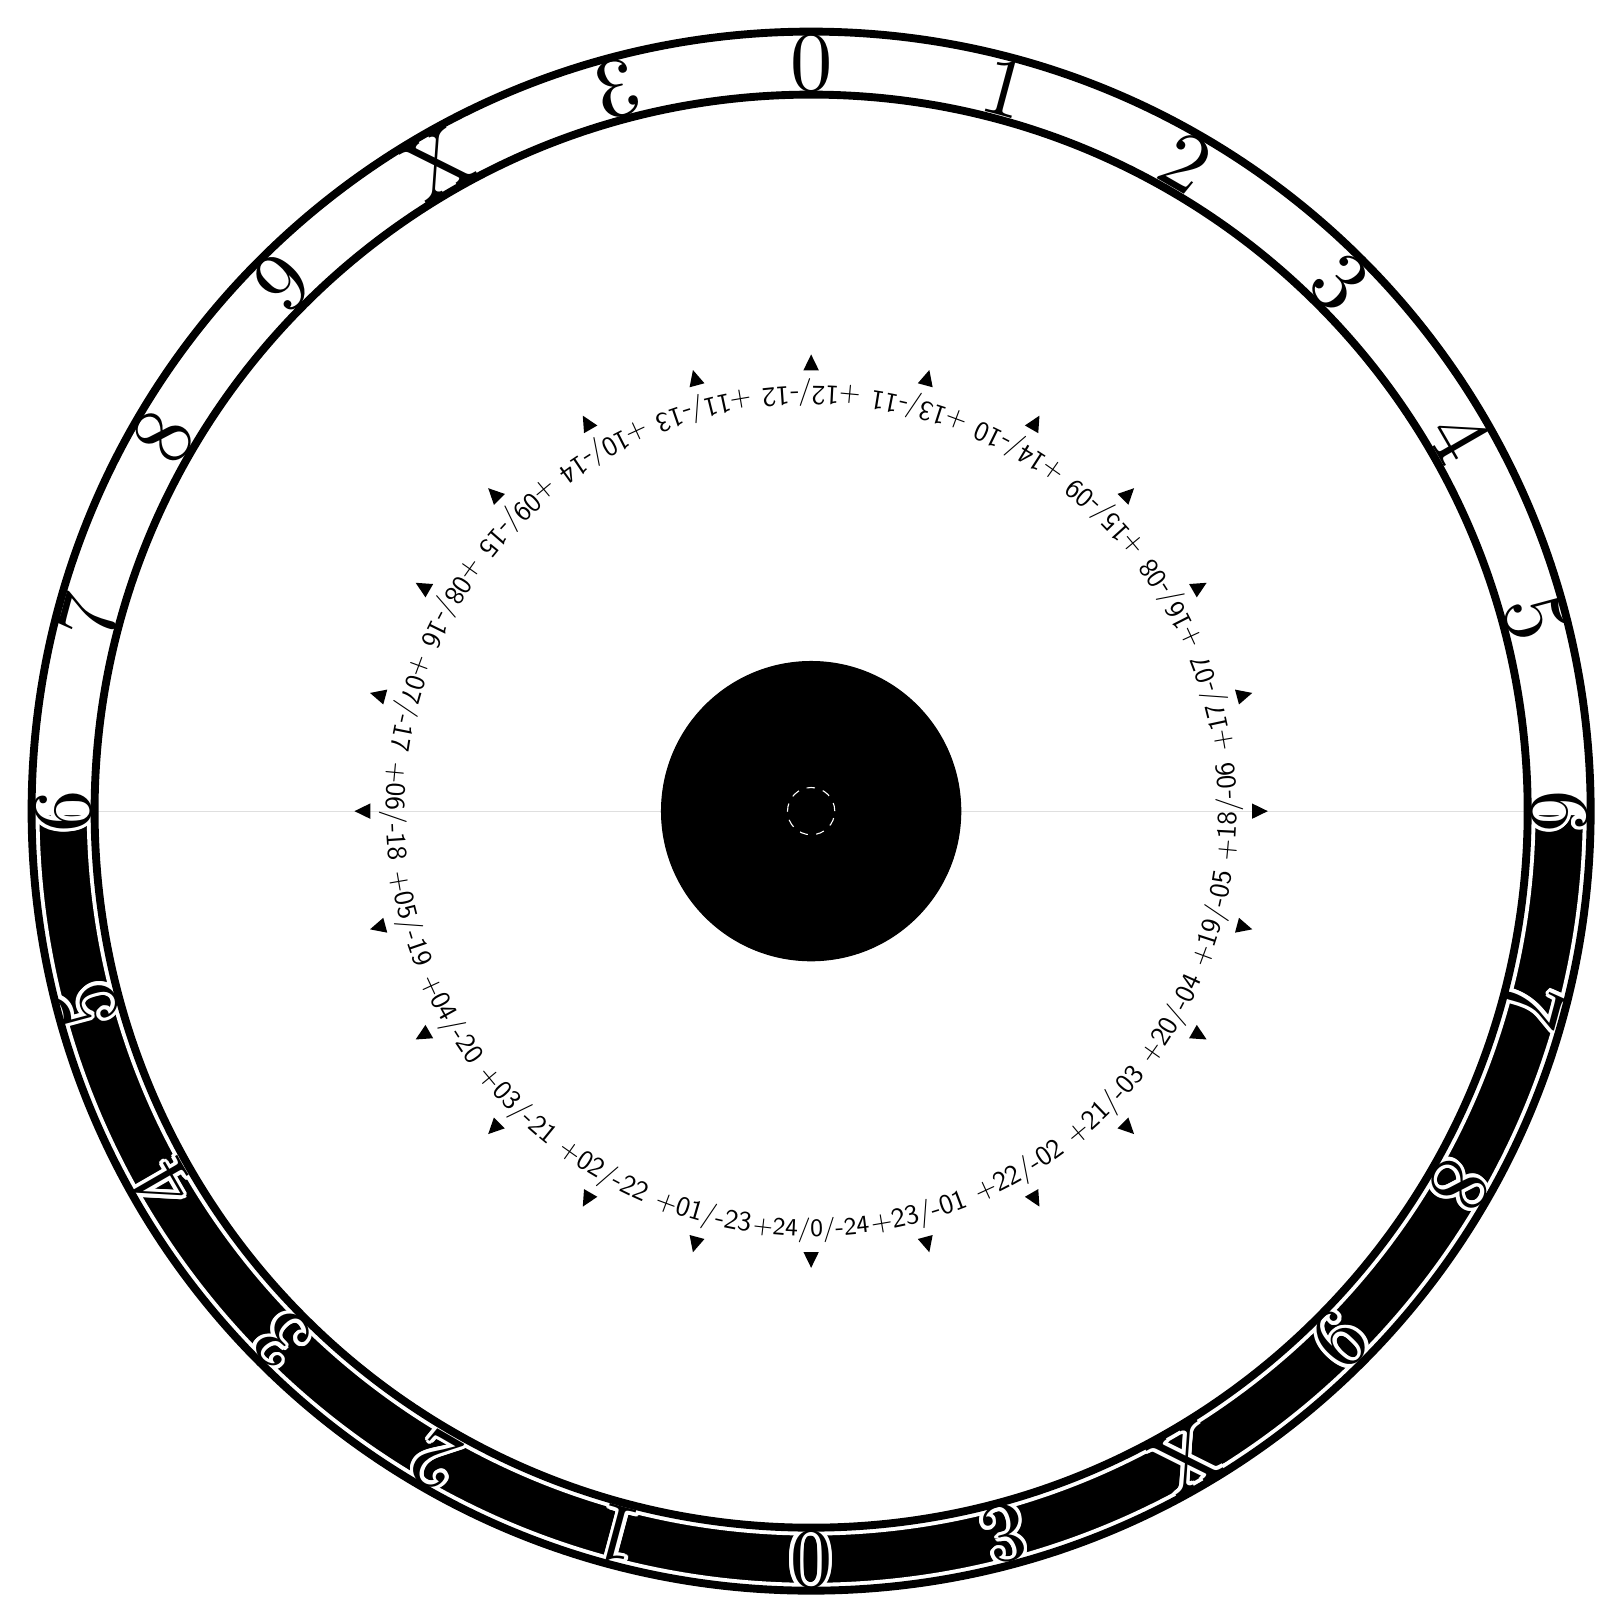
\begin{tikzpicture}
    % BORDER
    % \draw[dashed] (-100mm,-100mm) rectangle (100mm,100mm);
    \draw[fill] (0,0) circle [radius=18mm+1mm];
    \draw[dashed,white] (0,0) circle [radius=3mm];

    % INNER TIMEZONE ALIGNMENT
    % Timezones
    \foreach [count=\i] \plus/\minus in {%
            01/23,02/22,03/21,04/20,05/19,06/18,%
            07/17,08/16,09/15,10/14,11/13,12/12,%
            13/11,14/10,15/09,16/08,17/07,18/06,%
            19/05,20/04,21/03,22/02,23/01%
    } {
        \path[postaction={decorate,decoration={text align={center},text
            along path,text={|\sffamily|+\plus/-\minus}}}]
            (262.5-15*\i:54mm) arc (262.5-15*\i:277.5-15*\i:54mm);
        \fill (270+15*\i:58mm) -- (271+15*\i:56mm) -- (269+15*\i:56mm);
    }
    \path[postaction={decorate,decoration={text align={center},text
        along path,text={|\sffamily\small|+24/0/-24}}}]
        (262.5:54mm) arc (262.5:277.5:54mm);
    \fill (270:58mm) -- (271:56mm) -- (269:56mm);
    
    % OUTER RIM
    % Background
    \draw[fill=black,draw=white,line width=0.9mm+0.1mm]
        (180:91.5mm) -- (180:98.5mm) arc (180:360:98.5mm)
        (360:98.5mm) -- (360:91.5mm) arc (360:180:91.5mm);
    % Numerals
    \contourlength{0.15mm} % set to one 3rd (scale) of the desired width
    \foreach \angle/\label/\xscale in {%
            270/0/1,255/1/1,240/2/1,225/3/1,210/4/1,195/5/1,%
            180/6/1,165/7/1,150/8/1,135/9/1,120/X/1,105/3/-1%
    } {
        \node[rotate=\angle-90,scale=3.05,inner sep=0pt,xscale=\xscale]
            at (\angle:95mm-.22mm) {\contour{white}{\label}};
        \node[rotate=\angle+90,scale=3.05,inner sep=0pt,xscale=\xscale]
            at (\angle-180:95mm-.22mm) {\contour{white}{\label}};
    }
    % Borders
    \draw [line width=1mm] (0,0) circle [radius=100mm-1mm];
    \draw [line width=1mm] (0,0) circle [radius=90mm+1mm];

\end{tikzpicture}
        
\end{document}
